\documentclass[handout,9pt]{beamer}
%\documentclass[10pt]{beamer}
%\documentclass[draft, 10pt]{beamer}

%\mode<handout>{\beamertemplatesolidbackgroundcolor{black!5}}

 % \textheight 7cm
 %\doublespace
 %\oddsidemargin -1.5cm
 % \evensidemargin +1.5cm
 % \textwidth 12cm
 % \topmargin 0cm

%%%%%\usepackage{times}

%================================================================
\usepackage{ifthen}
\usepackage{color,amsmath,amsfonts,amssymb,epsfig,hyperref,graphicx}
\usepackage{dsfont}
\usepackage[latin1]{inputenc}
\usepackage[T1]{fontenc}
\usepackage[english]{babel}
\usepackage{fancyhdr}
%\usepackage{media9}
\usepackage{tikz}
%\usepackage{pgfplots}

%\usepackage{animate}
%\usepackage{multimedia}
\usepackage{everypage}
\usepackage[absolute,overlay]{textpos}
\usepackage{tikz}

\definecolor{enstrouge}{RGB}{212,65,84}
\definecolor{liteorange}{RGB}{235,226,52}
\definecolor{greenNoise}{RGB}{243,42,255}
\definecolor{LightRed}{rgb}{0.75,0.0325,0}
\definecolor{LightGrey}{rgb}{0.95,0.95,0.95}
\definecolor{Peach}{rgb}{0.98,0.49,0.25}
\definecolor{BurntOrange}{rgb}{0.79,0.37,0}
\definecolor{LightYellow}{rgb}{1,1,0.92}

\definecolor{litegreen}{RGB}{200,255,200}
\definecolor{enstorange}{RGB}{255,214,10}
\definecolor{enstrouge}{RGB}{212,65,84}
\definecolor{grey}{RGB}{204,204,204}
\definecolor{blue}{RGB}{0,0,255}
\definecolor{almostblack}{RGB}{100,100,100}
\definecolor{violet}{rgb}{0.4,0,0.4}
\definecolor{BurntOrange}{rgb}{0.79,0.37,0}
\definecolor{cyan}{RGB}{0,255,255}
\definecolor{magenta}{RGB}{243,42,255}


%================================================================
\mode<presentation> {
  %== theme
% Antibes, Berlin, Bergen, Berkeley,
% Boadilla, boxes, Copenhagen, Darmstadt, Dresden
% Frankfurt, Goettingen, Hannover, Ilmenau, JuanLesPins
% Luebeck, Madrid, Malmoe, Marburg, Montpellier, PaloAlto
% Pittsburgh, Rochester, Singapore, Szeged, Warsaw
  \usetheme{Copenhagen}%[width=0.18\linewidth,]
%%== colortheme
%%albatross, beetle, crane, dolphin, ove, fly, lily
%% orchid, rose, seagull, seahorse, sidebartab, whale
  \usecolortheme{rose}
  % \useoutertheme contient la pose du logo
  %\useoutertheme{default}
  \setbeamercovered{transparent}
}
\setbeamercolor{sidebar}{bg= enstrouge}
\setbeamercolor{structure}{fg= orange}
\setbeamercolor{alerted text}{fg=blue}

\usefonttheme[onlymath]{serif}
%=======================================
\setbeamerfont{page number in head/foot}{size=\large}
 \setbeamercolor{background canvas}{bg=LightYellow} 
 \setbeamertemplate{footline}[frame number]
 
%\pagestyle{fancy}
% \lhead[]{}
% \chead[]{}
% \rhead[]{}
% \lfoot[]{\includegraphics[scale=0.05]{\DIRLOGO/telecomparis}}
% \cfoot[]{\insertframenumber/\inserttotalframenumber}
% \rfoot[]{}

%======================================================================
%=============== NEW COMMANDS =========================================

\newcommand{\figsstit}[2]{
\begin{figure}[hbtp]
\centerline{
    \hbox{ \epsfig{figure={#1}, scale=#2} }
}
\end{figure}}
%===========================
\newcommand{\figscale}[4]{
\begin{figure}[hbtp]
\centerline{
    \hbox{ \epsfig{figure={#1}, scale=#4} }
}
\begin{center}
\parbox{11 cm}
{
    \caption{\protect\small\it  {#2}}
    \label {#3}
}
\end{center}
\end{figure}}
%===========================
\newcommand{\figdims}[5]{
\begin{figure}[hbtp]
\centerline{
    \hbox{ \epsfig{figure={#1}, height=#4cm, width=#5cm} }
}
\begin{center}
\parbox{10cm}
{
    \caption{\protect\small\it  {#2}}
    \label {#3}
}
\end{center}
\end{figure}}
%======================== \def =================
\def\with{\quad \text{with}\quad}
\def\where{\quad \text{where}\quad}
\def\and{\quad \text{and}\quad}
\def\gandl{\renewcommand\arraystretch{0.5}\begin{array}{c}H_{1}\\>\\<\\H_{0}\end{array}}
\def\GLRT{\ensuremath{\text{GLRT}}}
\def\GLRTdet{\ensuremath{\text{GLRT-det}}}
\def\GLRTstoEG{\ensuremath{\text{GLRT-sto-EG}}}
\def\GLRTstoVG{\ensuremath{\text{GLRT-sto-VG}}}
\def\m2{m$^2$}
\def\Fstat{{F\text{-stat}}}

\def\MSC{\text{MSC}}
\def\hMSC{\widehat{\text{MSC}}}

\def\simas{\stackrel{\mathrm{asympt.}}{\sim}}
\def\simiid{\stackrel{\mathrm{i.i.d.}}{\sim}}

% \def\linetext{\noindent
%       \makebox[\textwidth]{\color{orange}
%       {\rule{\textwidth}{1pt}}}}

 \def\linetext{\noindent{\color{orange}\rule{\textwidth}{1pt}
       \\[\dimexpr-\baselineskip+1mm+0pt]
                \rule{\textwidth}{0.5pt}}}

\def\linepaper{\noindent{\color{orange}\rule{\paperwidth}{1pt}
       \\[\dimexpr-\baselineskip+1mm+0pt]
                \rule{\paperwidth}{0.5pt}}}


%==================================================
\newcommand\algo[1]%
{
    \begin{center} %
    \begin{tabular} {||p{10 cm}l ||}%
    \hline
               #1 &  \\
    \hline
    \end{tabular}
    \vspace{12pt}
    \end{center}
}
\def\uB{\underline B}
\def\uD{\underline D}
\def\ur{\underline r}
\def\ux{\underline x}
\def\uX{\underline X}
\def\ug{\underline g}
\def\uw{\underline w}

\def\utheta{\underline \theta}
\def\uzeta{\underline \zeta}


\def\dx{\dot x}
\def\hx{\hat x}
\def\hy{\hat y}
\def\hX{\hat X}
\def\hY{\hat Y}
\def\tx{{\tilde x}}
\def\tX{{\tilde X}}
\def\cX{{\cal X}}


\def\soi{s_{\mathrm{soi}}}
\def\ns{s_{\mathrm{son}}}

\def\sut{\mathrm{UT}}
\def\sref{\mathrm{ref}}


\def\ssoi{\utheta_{\mathrm{soi}}}
\def\sns{\utheta_{\mathrm{son}}}
\def\degree{^{\circ}}

\def\cbullet{{\color{orange}\bullet}}

 \newcommand{\prob}[1]{\mathds{P}\left( #1 \right)}
 \newcommand{\esp}[1]{\mathds{E}\left[ #1 \right]}
 \newcommand{\espunder}[2]{\mathds{E}_{#1}\left[ #2 \right]}
 \newcommand{\var}[1]{\mathrm{var}\left( #1 \right)}
 \newcommand{\cov}[1]{\mathrm{Cov}\left( #1 \right)}
 \newcommand{\card}[1]{\left| #1 \right|}
 \newcommand\trace[1]{{\mathrm{Tr}} \left [ #1 \right] }
 \newcommand\diag[1]{{\mathrm{diag}} \left [ #1 \right] }
 \newcommand{\SNR}{\text{SNR}}
 \newcommand{\CRB}{\text{CRB}}
 \newcommand{\MLE}{\text{MLE}}
 \newcommand{\FIM}{\text{FIM}}
 \newcommand{\auc}{\text{AUC}}

\newenvironment{TAB}{\begin{table}[[hbt] \center \leavevmode}{\end{table}}
\newtheorem{propriete}{Propri\'{e}t\'{e} - \thepropriete}
\newtheorem{theoreme}{Th\'{e}or\`{e}me - \thetheoreme}
\newtheorem{definision}{D\'{e}finition - \thedefinision}
\newtheorem{exemple}{Exemple - \theexemple}
\newtheorem{lemme}{Lemme - \thelemme}


\newif\ifBIS \BISfalse 


%=========== LOGO par SLIDE =====================================
\pgfdeclareimage[height=0.6cm]{logoCTBTO}{logoctbto}

%%============================================================================
%\def\thesection{\arabic{section}}
%\def\thefigure{\arabic{figure}}
%\def\theequation{\arabic{equation}}
%\def\theexercice{\arabic{exercice}}
%\def\theequation{\arabic{exercice}.\arabic{equation}}
%%============================================================================
%\newcounter{auxiliaire}
%%%%%%%% comment
%\setcounter{auxiliaire}{\theenumi}
%\end{enumerate}
% TEXTE
%\begin{enumerate}
%\setcounter{enumi}{\theauxiliaire}
%%============================================================================
%\renewcommand\arraystretch{1.6}
%%============================================================================
%\begin{center}
%\renewcommand\arraystretch{1.8}
%\begin{tabular}{|l|l|p{6cm}|}
%\hline
%fonction &  expression & application
%\\
%\hline\hline
%\end{tabular}
%\end{center}
%%============================================================================
%============================================================================
%============= mise en page =================================================
% dans le bandeau inf\'{e}rieur

% Delete this, if you do not want the table of contents to pop up at
% the beginning of each subsection:
%\AtBeginSubsection[]
%{
%  \begin{frame}<beamer>
%    \frametitle{Outline}
%    \tableofcontents[currentsection,currentsubsection]
%  \end{frame}\pageblanche
%}

\setcounter{tocdepth}{1}

\graphicspath{{figures/}}


%%=======================================================
%================= TITRE ===============================
%============================================
\title{Evaluation of infrasound in-situ calibration method on a 3-month measurement campaign}
\author{
 Charbit M.$^{1}$, 
 Doury B.$^{2}$
 Marty J.$^{3}$,
%\\ \vspace{12pt}
%\parbox{20cm}{ 
%{\tiny  (1) maurice.charbit@CTBT.ORG, CTBTO},\\
%{\tiny (2) benoit.doury@CTBT.ORG, CTBTO}\\,
%{\tiny (3) julien.marty@CTBT.ORG, CTBTO} }\vspace{-24pt}
}

%================== debut ==============================
%=======================================================

% \logo{
% \colorbox{litegreen}{\makebox(352,18){\textcolor{black}
% {\normalsize Infrasound Technology Workshop 2015\hspace{10pt}\vspace{10pt}
%  { \hspace{+0.4cm}  \pgfuseimage{logoCTBTO}}}}}}
 \logo{\colorbox{litegreen}
 {\hspace{12pt}\normalsize\color{black}Infrasound Technology Workshop 2015
 \hspace{20pt}\pgfuseimage{logoCTBTO}}\vspace{-0.68cm}\hspace{-0.0cm}}


 \bibliographystyle{plain} 

\begin{document}
 \sloppy
%=======================================================
%=======================================================
%\begin{frame}
%\frametitle{Short outline}
% \tableofcontents
%\end{frame}

%=======================================================
%=======================================================
\begin{frame}
\maketitle
\end{frame}


 \section{Introduction}
%=======================================================
%=======================================================
\begin{frame}
 \frametitle{IMS study}
 In the framework of the calibration program, a study was conducted 
 with the following theoretical and practical results:
 \begin{itemize}
 \item
 closed form expression for the asymptotic probability distributions of the spectrum ratio which is the base of the estimation;
 \item
 sizing the statistic of test for the {\bf  magnitude square coherence (MSC)} level;
 \item
 introducing a weighted estimator of the {\bf system under test (SUT)} response based on the estimated value of 
the MSC;
 \item
 proposal of a filter bank analysis for the SUT estimation;
 \item
 providing a simple wind coherence model which explains an observed artefact of the {\bf noise reduction system} (NRS), in relation with the wind velocity;
 \item
{\bf \color{red} Evaluation on a measurement campaign at station IS26 during several months.}
 \end{itemize}
 
 
\end{frame}
%=======================================================
%=======================================================
%=======================================================
\begin{frame}
\frametitle{Measurement chain [Kramer and al., ITW2015]}


\begin{center}
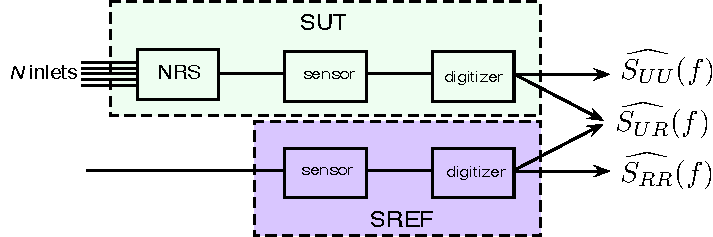
\includegraphics[scale=0.7]{fulltestbedIS26.pdf}
\end{center}



%\vspace{-24pt}
\begin{itemize}
\item
the objective is the calibration of the SUT, which consists of the NRS, the sensor and a digitizer, based on the knowledge of the 
  {\bf system of reference (SREF)};
\item
2 kinds of signals: acoustic and non acoustic (typically wind) with different ranges of velocity;
\item
non spatially coherent signals are called ``noise'';
\item
acoustic signals is spatially coherent, in all frequency band of interest, regarding the size of the SUT. 
\end{itemize}


\end{frame}
%=======================================================
%=======================================================
%=======================================================
\begin{frame}
\frametitle{Undetermined problem}
\begin{eqnarray*}
\left\{
\renewcommand\arraystretch{1.6}
\begin{array}{rcl}
s_{\sut}(t)&=&{\color{blue}h_{\sut}}(t)\star({\color{blue}s}(t)+{\color{blue}w_{\sut}}(t))
\\
s_{\sref}(t)&=&h_{\sref}(t)\star({\color{blue}\alpha}\times {\color{blue}s}(t)+{\color{blue}w_{\sref}}(t))
%\\
%\alpha&=&1
\end{array}\right.
\end{eqnarray*}
\begin{itemize}
\item
ill-posed problem because under-determinated: 4 unknowns for 2 observations;
\item
but with stationary and ``almost 0-noise'' time segments the problem is well-determined

\item
 the MSC provides a way to test ``almost 0-noise'' time segments;
\item
theoretical results show that, to get an accuracy of $\pm 5\%$ on the gain, we need an MSC value greater than $0.96$;
\item
but because only an estimate of the $\MSC$ is available, we have to threshold at about $0.98$. %for a confidence level of $90\%$ 
\end{itemize}
\end{frame}

%=======================================================
%=======================================================
\begin{frame}
\frametitle{Performing process}

\begin{center}
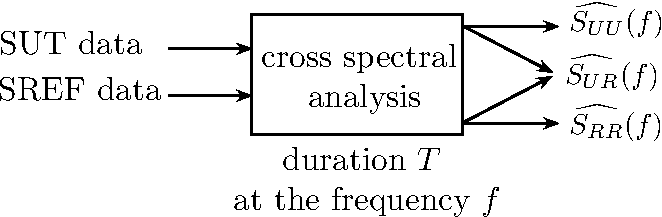
\includegraphics[scale=0.7]{processdetail.pdf}
\end{center}

\vspace{-0.5cm}

\begin{eqnarray*}
\left\{
\renewcommand\arraystretch{1.6}
\begin{array}{rcl}
s_{\sut}(t)&\approx&g_{\sut}(t)\star s(t) 
\\
s_{\sref}(t)&\approx&g_{\sref}(t)\star {\color{blue}\alpha} s(t)
%\\
%\alpha&=&1
\end{array}\right.
\end{eqnarray*}

For stationary and ``almost 0-noise'' time segments we have:
\begin{eqnarray*}
\widehat{G_{\mathrm{UT}}}(f)
\approx G_{\mathrm{ref}} \times
%\underbrace{
\color{red}\frac{\widehat{{S}_{\mathrm{UU}}}(f)}
                        {\widehat{{S}_{\mathrm{RU}}}(f)}
                        %}
%_{\color{red}\mathrm{spectrum}\, \mathrm{ratio}}
\end{eqnarray*}
if $\alpha<1$, we underestimate $G_{\sut}$.

%The product F x T is an index of accuracy. Therefore we can reduce the duration in high frequencies if necessary.

\end{frame}
%=======================================================
%=======================================================
%=======================================================
\begin{frame}
\frametitle{Manage the stationarity}

\begin{itemize}
\item
In relationship with the resolution but also to take into account  the lack of stationarity, we have considered a sequence of 6 durations in decreasing order with the frequency. A pre-filtering is also performed. %However we have noticed that the design is not critical.

%\item
%In the following results the filter bank reported on the figure has been used. 

\end{itemize}

     \figsstit{filterbank.pdf}{0.5}

\end{frame}
%=======================================================
%=======================================================
%=======================================================
\begin{frame}
\frametitle{NRS effect}

If $v$ denotes the wind velocity, the ratio $\dfrac{v}{f}$ can be interpreted as a ``wavelength'' [Alcoverro, al., JASA,
2002]. Therefore

%\bigskip

\begin{tabular}{clc}
\hspace{-1cm}
\begin{minipage}{6cm}
\begin{itemize}
\item
{\color{red}at very low frequency}, 
{ the wind appears as spatially coherent for all SUT/SREF inlets. Therefore everything occurs as there is NO noise, and the MSC is almost 1},
\item
{\color{red}at high frequency},  
{the wind appears as spatially NON coherent. Therefore the NRS plays its role to reduce the noise},
\item
{\color{red}around $0.8$ Hz}, 
{a small part of the wind appears as  spatially coherent for a few NRS inlets. Therefore a small dip artefact is observed}.
\end{itemize}
\end{minipage}
&
\begin{minipage}{7.5cm}
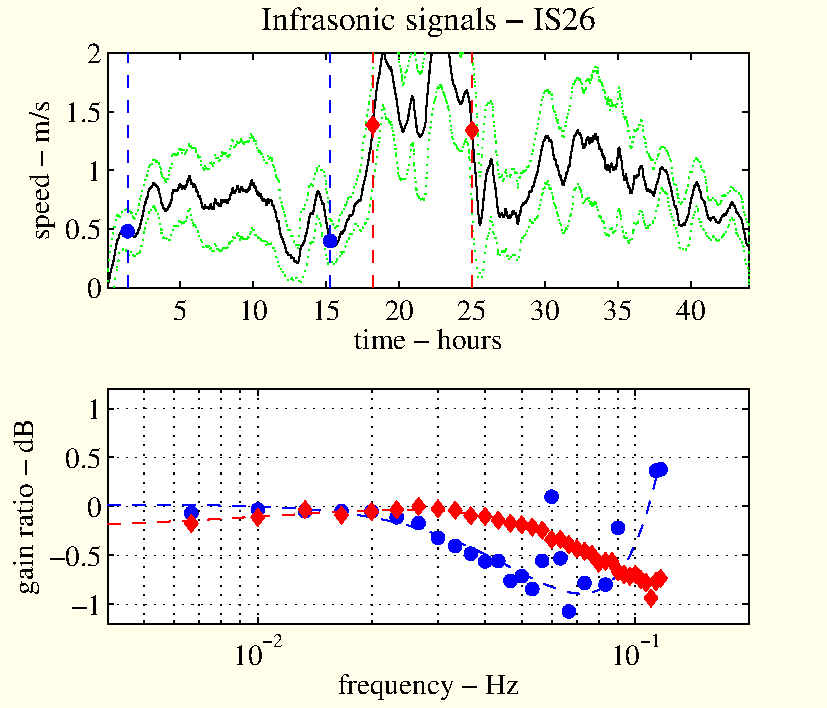
\includegraphics[scale=0.45]{twospeedster.pdf}
\end{minipage}
\end{tabular}
\end{frame}

%=======================================================
\section{Campaign measurement results}
%=======================================================
%=======================================================
\begin{frame}
\frametitle{Deployment [A.Kramer, al., ITW2015]}
\begin{itemize}
\item
8 SUTs with 18 meter wind noise reduction system, each of them with 96 inlets;
\item
8 SREFs have been deployed on May 2015;
\item
each reference sensor has been calibrated in the lab;
\item
wind velocity and direction are available on H1.
\end{itemize}
\end{frame}

%=======================================================
%=======================================================
\begin{frame}
\frametitle{PTS requirements}
\framebox[11cm]{
\begin{minipage}{10cm}
PTS specifications are:
\begin{itemize}
\item
bandwidth $[0.02 - 4]$ Hz;
 \item
$\pm 5\%$ on the response magnitude, i.e. $\pm 0.43$ in dB scale;
\item
the calibration is required at least once a year;
 \item
no requirement  on the phase but $\ldots$ $\pm 5\degree$ as for seismic requirements.
\end{itemize}
\end{minipage}
}
\end{frame}


%=======================================================
%=======================================================
\begin{frame}
\frametitle{Averaging on a few months}
\begin{tabular}{c||c}
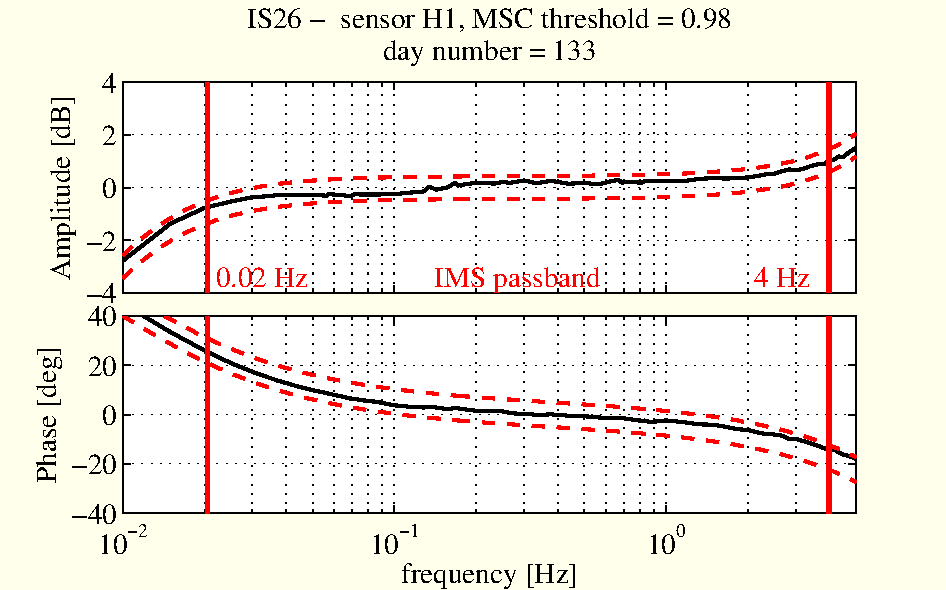
\includegraphics[scale=0.35]{3monthsonIS26SUTboxplot1.pdf}
&
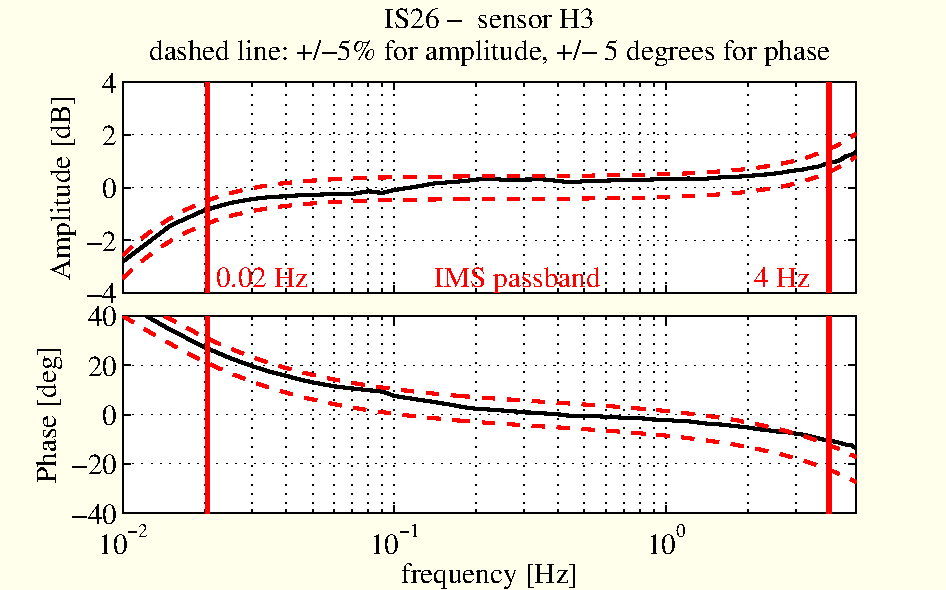
\includegraphics[scale=0.35]{3monthsonIS26SUTboxplot3.pdf}
\\
\hline\hline
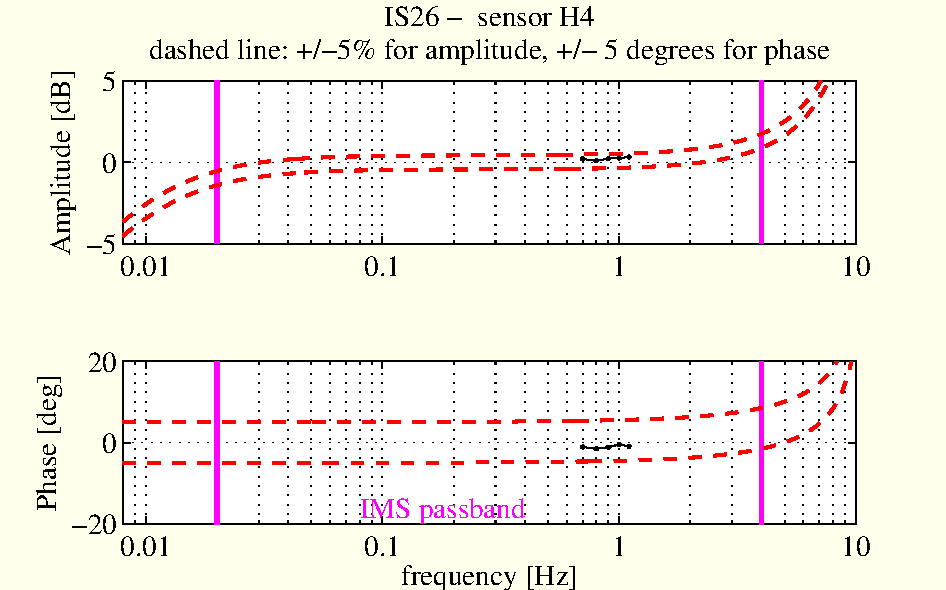
\includegraphics[scale=0.35]{3monthsonIS26SUTboxplot4.pdf}
&
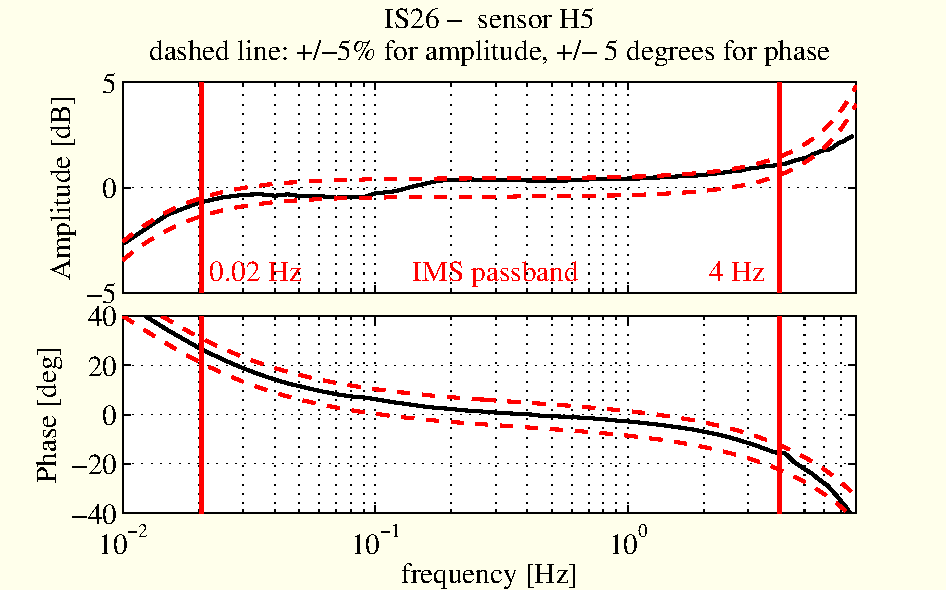
\includegraphics[scale=0.35]{3monthsonIS26SUTboxplot5.pdf}
\end{tabular}
\end{frame}

%=======================================================
%=======================================================
\begin{frame}
\frametitle
{Temporal stability of successive gains at $1$ Hz averaged on $2$ days}
\begin{tabular}{c||c}
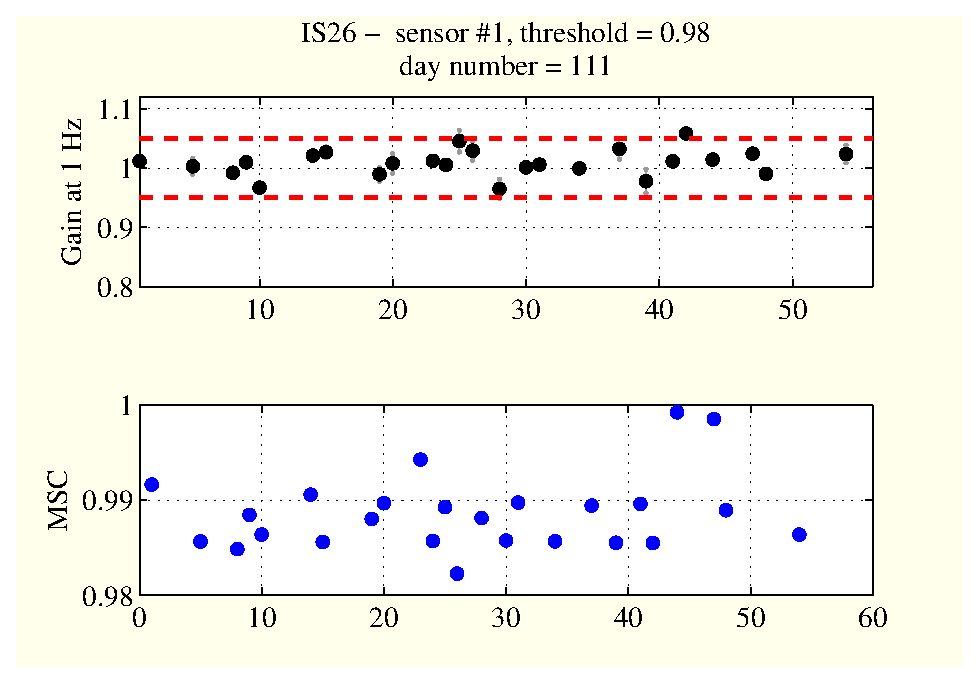
\includegraphics[scale=0.3]{evolutionon1atfreq1.eps}
&
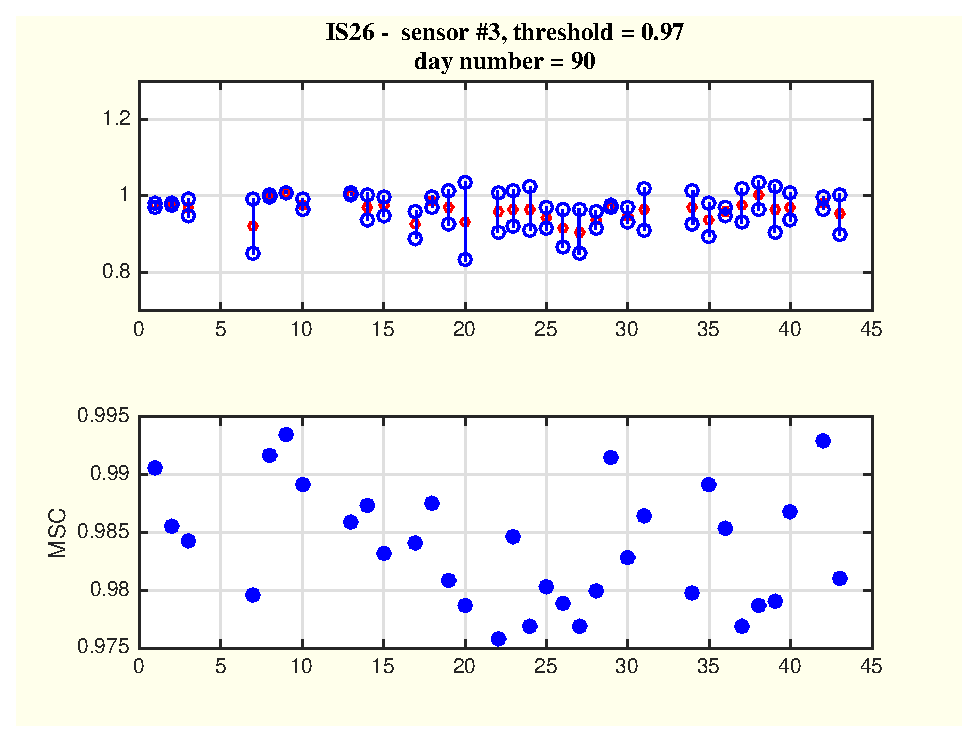
\includegraphics[scale=0.3]{evolutionon3atfreq1.eps}
\\
\hline\hline
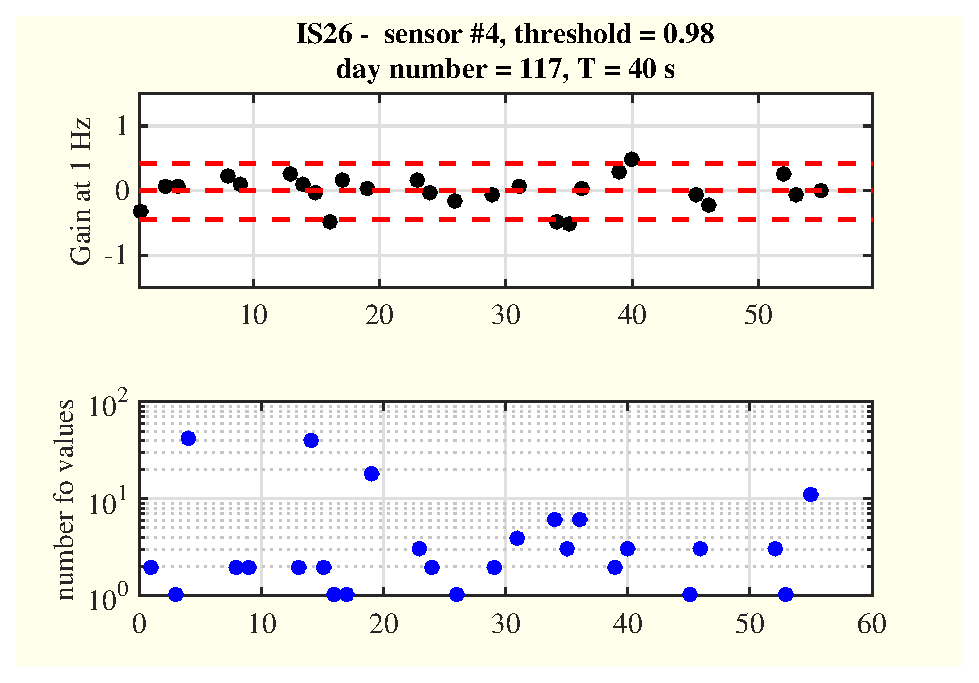
\includegraphics[scale=0.3]{evolutionon4atfreq1.eps}
&
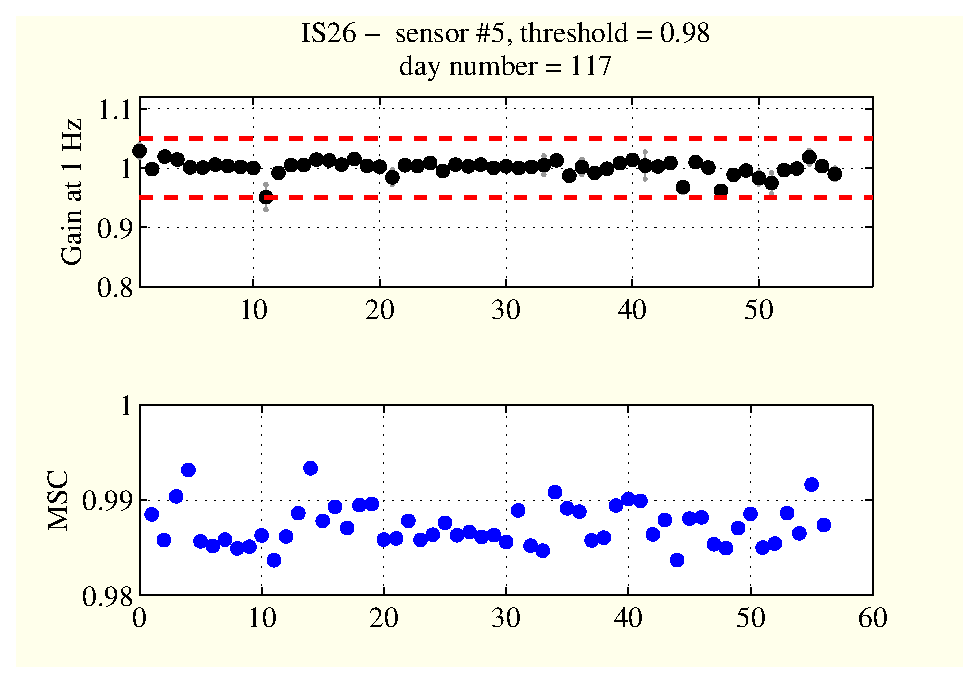
\includegraphics[scale=0.3]{evolutionon5atfreq1.eps}
\end{tabular}
\end{frame}

%=======================================================
%=======================================================
\begin{frame}
\frametitle{Conclusions}

%\framebox[11cm]{
%\begin{minipage}{10cm}
%PTS specifications are:
%\begin{itemize}
%\item
%bandwidth $[0.02 - 4]$ Hz;
% \item
%$\pm 5\%$ on the response magnitude; more specifically the calibration is required once a year;
% \item
%no requirement  on the phase but $\ldots$ $\pm 5\degree$ has been considered.
%\end{itemize}
%\end{minipage}
%}
\framebox[11cm]{
\begin{minipage}{10cm}
Conclusions:
\begin{itemize}
\item
The numerical results obtained on a large campaign of measurements fully validate the calibration method;
\item
The experimental results obtained by couples of 2 days show a high stability in full agreement with the PTS requirements;
%\item
%the small dip present in the curve stays in the PTS requirements and is proved to be an artefact of the NRS and not a default of the SUT or the %measurement process.
\end{itemize}
\end{minipage}
}
\end{frame}

%=======================================================
%=======================================================
 \begin{frame}
\begin{center}
{\large THANKS FOR YOUR ATTENTION}
\end{center}
\end{frame}

%=======================================================
%=======================================================
\begin{frame}\frametitle{NRS effect simulation}
\begin{center}
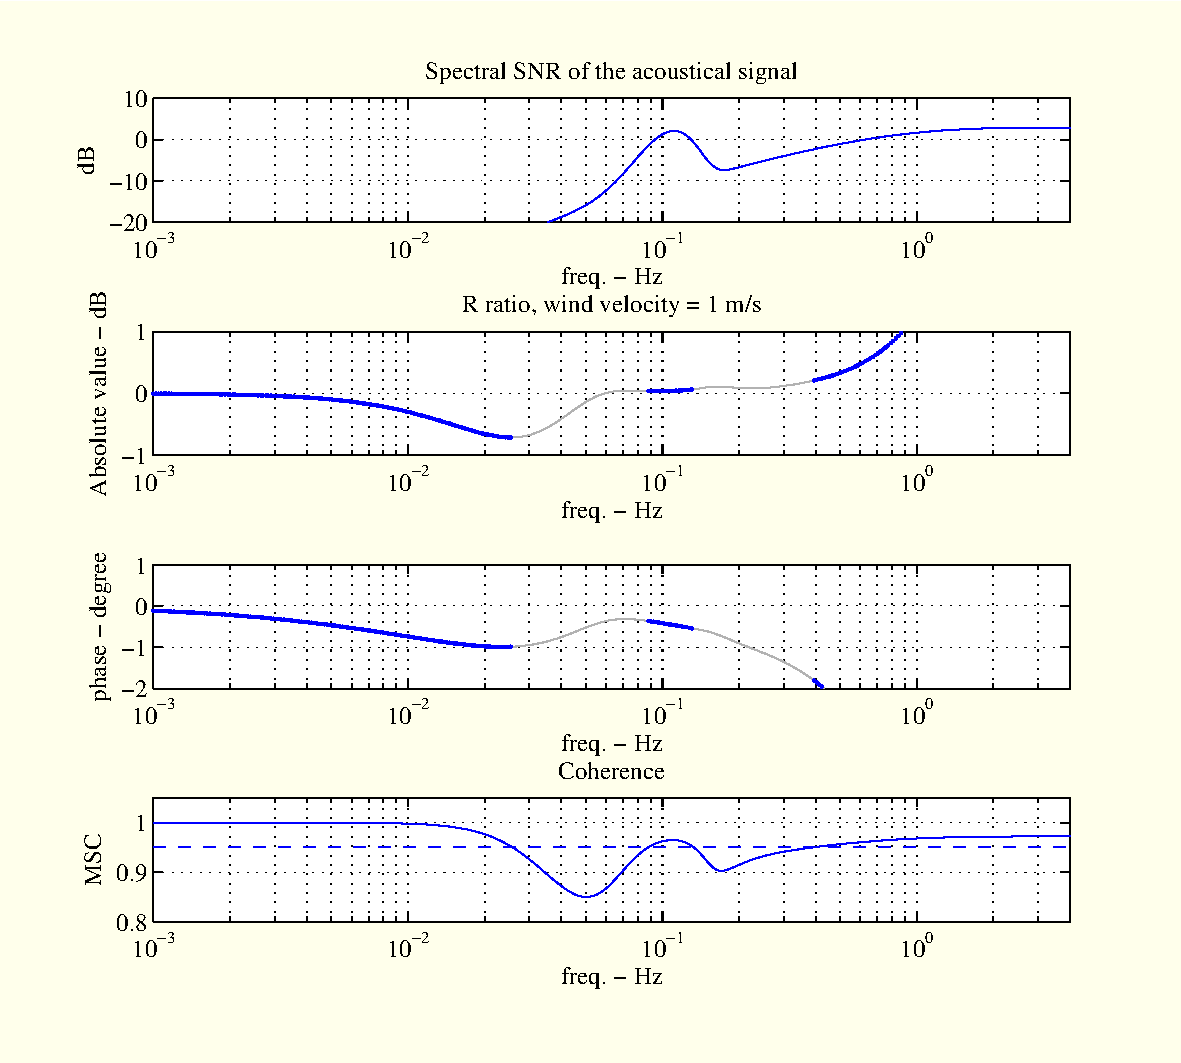
\includegraphics[scale=0.36]{GonH.pdf}
\end{center}
\end{frame}
%=======================================================
%=======================================================
\begin{frame}\frametitle{Rks}
{\tiny
\begin{center}
\hspace{-0.8 cm}
\fbox{$X_1,\cdots,X_{2000}$}\ \fbox{$X_{2001},\cdots,X_{4000}$}\ %
\fbox{$X_{4001},\cdots,X_{6000}$}\ \fbox{$X_{6001},\cdots,X_{8000}$}\
%
\fbox{$X_{8001},\cdots,X_{10000}$} \\
\hspace{-1. cm}
\fbox{$X_{1001},\cdots,X_{3000}$}\ \fbox{$X_{3001},\cdots,X_{5000}$}\
%
\fbox{$X_{5001},\cdots,X_{7000}$}\ \fbox{$X_{7001},\cdots,X_{9000}$}
\end{center}
}
\begin{itemize}
\item
If we have $N=2000$ samples the resolution is  $F_s/N=0.01$ Hz. 
Therefore there is a possibility to decimate if the bandwidth is $B<0.01$.
But for sake of simplicity, we keep the common value $F_s$ to all filters of the bank (no decimation).
\item
For each frequency bin, an averaging is applied on the $L=9$ segments. If a few number of bins is required the fft algorithm is not needed.
\end{itemize}
\end{frame}
%=======================================================
%=======================================================


\end{document}

